% questions.tex —— 2013 年·北京卷·文科 · 题目内容片段（无答案）
% 由 tools/generate_projects.py 依来源总账自 2013/2013_数学真题_北京文_试题.md 生成，勿手改（改源 MD 后重跑）


\begin{gknotice}
\textbf{来源说明}：本题面依据固定源 PDF 的两页 A3 题面逐题转录，原卷印刷页码为 789—790。第 789 面为选择题 1—8、填空题 9—14、解答题 15—16，第 790 面为解答题 17—20。原卷无选做栏。

\textbf{解析归属}：固定源不附答案或解析；配套答案与解析均由本库按本题面独立复算。

\textbf{图形说明}：第 6 题程序框图、第 8 题正方体、第 10 题三视图、第 16 题空气质量指数趋势图、第 17 题四棱锥，均由项目内 TikZ 矢量源重绘。
\end{gknotice}

\gkpart{一、选择题}

\begin{question}
\gkti{1}已知集合 $A=\{-1,0,1\}$，$B=\{x\mid-1\leqslant x<1\}$，则 $A\cap B=$\mbox{（　　）}

（A）$\{0\}$；（B）$\{-1,0\}$；（C）$\{0,1\}$；（D）$\{-1,0,1\}$。

\end{question}
\begin{question}
\gkti{2}设 $a$，$b$，$c\in\mathbf R$，且 $a>b$，则\mbox{（　　）}

（A）$ac>bc$；（B）$\dfrac1a<\dfrac1b$；（C）$a^2>b^2$；（D）$a^3>b^3$。

\end{question}
\begin{question}
\gkti{3}下列函数中，既是偶函数又在区间 $(0,+\infty)$ 上单调递减的是\mbox{（　　）}

（A）$y=\dfrac1x$；（B）$y=\mathrm e^{-x}$；（C）$y=-x^2+1$；（D）$y=\lg|x|$。

\end{question}
\begin{question}
\gkti{4}在复平面内，复数 $\mathrm i(2-\mathrm i)$ 对应的点位于\mbox{（　　）}

（A）第一象限；（B）第二象限；（C）第三象限；（D）第四象限。

\end{question}
\begin{question}
\gkti{5}在 $\triangle ABC$ 中，$a=3$，$b=5$，$\sin A=\dfrac13$，则 $\sin B=$\mbox{（　　）}

（A）$\dfrac15$；（B）$\dfrac59$；（C）$\dfrac{\sqrt5}3$；（D）$1$。

\Needspace{0.4\textheight}
\end{question}
\begin{question}
\gkti{6}执行如图所示的程序框图，输出的 $S$ 值为\mbox{（　　）}
\nopagebreak[4]
\begin{center}% 2013 年北京卷文科第 6 题：程序框图。
% 来源 PDF：普通高考/2013/2013北京文.pdf，第 1 页（印面 789）左栏。
% 流程：开始 → i=0,S=1 → S=(S^2+1)/(2S+1) → i=i+1 → i≥2?
%       是：输出 S → 结束；否：向右引出后回到 S 赋值框上方。
\begin{tikzpicture}[font=\footnotesize, >=Stealth, line width=0.45pt,
  term/.style={draw, rounded corners=6pt, minimum height=1.8em, inner xsep=9pt},
  io/.style={draw, trapezium, trapezium left angle=70, trapezium right angle=110,
             minimum height=1.8em, inner xsep=6pt},
  box/.style={draw, minimum height=1.9em, inner xsep=6pt},
  dec/.style={draw, diamond, aspect=2.4, inner sep=1pt}]
  \node[term] (start) at (0,0) {开始};
  \node[box] (init) at (0,-1.05) {$i=0$，$S=1$};
  \node[box] (assign) at (0,-2.35) {$S=\dfrac{S^2+1}{2S+1}$};
  \node[box] (inc) at (0,-3.70) {$i=i+1$};
  \node[dec] (cond) at (0,-5.05) {$i\geqslant2$};
  \node[io] (out) at (0,-6.40) {输出 $S$};
  \node[term] (end) at (0,-7.50) {结束};
  \draw[->] (start) -- (init);
  \draw[->] (init) -- (assign);
  \draw[->] (assign) -- (inc);
  \draw[->] (inc) -- (cond);
  \draw[->] (cond) -- node[right] {是} (out);
  \draw[->] (out) -- (end);
  % 循环支路：从判断框右侧引出，上行后折回 S 赋值框顶边
  \coordinate (r1) at ($(cond.east)+(2.3,0)$);
  \coordinate (up) at ($(assign.north)+(0,0.45)$);
  \draw (cond.east) -- node[above] {否} (r1) -- (r1 |- up) -- (0.55,0 |- up);
  \draw[->] (0.55,0 |- up) -- (0.55,0 |- assign.north);
\end{tikzpicture}
\end{center}
\nopagebreak[4]
（A）$1$；（B）$\dfrac23$；（C）$\dfrac{13}{21}$；（D）$\dfrac{610}{987}$。

\end{question}
\begin{question}
\gkti{7}双曲线 $x^2-\dfrac{y^2}m=1$ 的离心率大于 $\sqrt2$ 的充分必要条件是\mbox{（　　）}

（A）$m>\dfrac12$；（B）$m\geqslant1$；（C）$m>1$；（D）$m>2$。

\Needspace{0.4\textheight}
\end{question}
\begin{question}
\gkti{8}如图，在正方体 $ABCD-A_1B_1C_1D_1$ 中，$P$ 为对角线 $BD_1$ 的三等分点，$P$ 到各顶点的距离的不同取值有\mbox{（　　）}
\nopagebreak[4]
\begin{center}% 2013 年北京卷文科第 8 题：正方体 ABCD-A1B1C1D1 与对角线 BD1 的三等分点 P。
% 来源 PDF：普通高考/2013/2013北京文.pdf，第 1 页（印面 789）中栏上方。
% 可见棱用实线，被遮住的 PA 类棱用虚线；BD1 为点划线，P 为其三等分点。
\begin{tikzpicture}[font=\footnotesize, line width=0.45pt]
  \coordinate (A)  at (0,0);
  \coordinate (B)  at (3,0);
  \coordinate (C)  at (4.3,1.3);
  \coordinate (D)  at (1.3,1.3);
  \coordinate (A1) at (0,3);
  \coordinate (B1) at (3,3);
  \coordinate (C1) at (4.3,4.3);
  \coordinate (D1) at (1.3,4.3);
  % 可见棱
  \draw (A) -- (B) -- (C) -- (C1) -- (B1) -- (B);
  \draw (A1) -- (B1) -- (C1) -- (D1) -- cycle;
  \draw (A1) -- (A);
  % 被遮挡的棱
  \draw[dashed] (A) -- (D) -- (C);
  \draw[dashed] (D) -- (D1);
  % 对角线 BD1 与三等分点 P
  \draw[densely dotted] (B) -- (D1);
  \coordinate (P) at ($(B)!0.3333!(D1)$);
  \fill (P) circle (1.5pt);
  \node[right] at (P) {$P$};
  % 顶点标注
  \node[below left]  at (A)  {$A$};
  \node[below right] at (B)  {$B$};
  \node[right]       at (C)  {$C$};
  \node[above left]  at (D)  {$D$};
  \node[left]        at (A1) {$A_1$};
  \node[right]       at (B1) {$B_1$};
  \node[right]       at (C1) {$C_1$};
  \node[above left]  at (D1) {$D_1$};
\end{tikzpicture}
\end{center}
\nopagebreak[4]
（A）$3$ 个；（B）$4$ 个；（C）$5$ 个；（D）$6$ 个。

\end{question}
\begingroup
\renewcommand{\gkpart}[1]{\Needspace{0.3\textheight}\subsection*{#1}\nopagebreak}
\gkpart{二、填空题}
\endgroup

\begin{question}
\gkti{9}若抛物线 $y^2=2px$ 的焦点坐标为 $(1,0)$，则 $p=$\gkblank{}；准线方程为\gkblank{}。

\Needspace{0.4\textheight}
\end{question}
\begin{question}
\gkti{10}某四棱锥的三视图如图所示，该四棱锥的体积为\gkblank{}。
\nopagebreak[4]
\begin{center}% 2013 年北京卷文科第 10 题：四棱锥的三视图。
% 来源 PDF：普通高考/2013/2013北京文.pdf，第 1 页（印面 789）中栏。
% 正视图底边 2+1=3、高 1；侧视图底边 1+2=3、高 1；俯视图为边长 3 的正方形，
% 内部四条线汇聚于顶点的投影（距左边 2、距上边 1）。
\begin{tikzpicture}[font=\footnotesize, line width=0.45pt, >=Stealth]
  % 正（主）视图
  \draw (0,0) -- (3,0) -- (2,1) -- cycle;
  \draw[|<->|] (0,-0.30) -- (1.95,-0.30) node[midway,below] {$2$};
  \draw[|<->|] (2.05,-0.30) -- (3,-0.30) node[midway,below] {$1$};
  \foreach \x in {0,2,3} \draw (\x,-0.18) -- (\x,-0.42);
  \node at (1.5,-1.0) {正（主）视图};
  % 高 1（正视图与侧视图之间）
  \draw[gray!70] (2,1) -- (3.55,1);
  \draw[gray!70] (3,0) -- (3.55,0);
  \draw[|<->|] (3.42,0) -- (3.42,1) node[midway,left] {$1$};
  % 侧（左）视图
  \draw (4.5,0) -- (7.5,0) -- (5.5,1) -- cycle;
  \draw[|<->|] (4.5,-0.30) -- (5.45,-0.30) node[midway,below] {$1$};
  \draw[|<->|] (5.55,-0.30) -- (7.5,-0.30) node[midway,below] {$2$};
  \foreach \x in {4.5,5.5,7.5} \draw (\x,-0.18) -- (\x,-0.42);
  \node at (6.0,-1.0) {侧（左）视图};
  % 俯视图
  \draw (1.2,-1.7) rectangle (4.2,-4.7);
  \coordinate (Q) at (3.2,-2.7);
  \draw (1.2,-1.7) -- (Q);
  \draw (4.2,-1.7) -- (Q);
  \draw (1.2,-4.7) -- (Q);
  \draw (4.2,-4.7) -- (Q);
  \node at (2.7,-5.15) {俯视图};
\end{tikzpicture}
\end{center}
\nopagebreak[4]
\end{question}
\begin{question}
\gkti{11}若等比数列 $\{a_n\}$ 满足 $a_2+a_4=20$，$a_3+a_5=40$，则公比 $q=$\gkblank{}，前 $n$ 项和 $S_n=$\gkblank{}。

\end{question}
\begin{question}
\gkti{12}设 $D$ 为不等式组 $\begin{cases}x\geqslant0,\\2x-y\leqslant0,\\x+y-3\leqslant0\end{cases}$ 表示的平面区域，区域 $D$ 上的点与点 $(1,0)$ 之间的距离的最小值为\gkblank{}。

\end{question}
\begin{question}
\gkti{13}函数
\nopagebreak[4]
\[f(x)=\begin{cases}\log_{\frac12}x,&x\geqslant1,\\2^x,&x<1\end{cases}\]
的值域为\gkblank{}。

\end{question}
\begin{question}
\gkti{14}已知点 $A(1,-1)$，$B(3,0)$，$C(2,1)$。若平面区域 $D$ 由所有满足 $\overrightarrow{AP}=\lambda\overrightarrow{AB}+\mu\overrightarrow{AC}$（$1\leqslant\lambda\leqslant2$，$0\leqslant\mu\leqslant1$）的点 $P$ 组成，则 $D$ 的面积为\gkblank{}。

\end{question}
\begingroup
\renewcommand{\gkpart}[1]{\Needspace{0.3\textheight}\subsection*{#1}\nopagebreak}
\gkpart{三、解答题}
\endgroup

\begin{question}
\gkti{15}已知函数 $f(x)=(2\cos^2x-1)\sin2x+\dfrac12\cos4x$。

（1） 求 $f(x)$ 的最小正周期及最大值；

（2） 若 $\alpha\in\left(\dfrac{\pi}2,\pi\right)$，且 $f(\alpha)=\dfrac{\sqrt2}2$，求 $\alpha$ 的值。

\Needspace{0.4\textheight}
\end{question}
\begin{question}
\gkti{16}下图是某市 $3$ 月 $1$ 日至 $14$ 日的空气质量指数趋势图，空气质量指数小于 $100$ 表示空气质量优良，空气质量指数大于 $200$ 表示空气重度污染。某人随机选择 $3$ 月 $1$ 日至 $3$ 月 $13$ 日中的某一天到达该市，并停留 $2$ 天。
\nopagebreak[4]
\begin{center}% 2013 年北京卷文科第 16 题：3 月 1 日至 14 日空气质量指数趋势图。
% 来源 PDF：普通高考/2013/2013北京文.pdf，第 1 页（印面 789）右栏（与理科第 16 题同一张图）。
% 14 个数据点（600 dpi 原页逐个核对）：86，25，57，143，220，160，40，
% 217，160，121，158，86，79，37。
\begin{tikzpicture}[font=\scriptsize, >=Stealth, line width=0.45pt,
  x=0.79cm, y=0.026cm]
  % 坐标轴
  \draw[->] (0,0) -- (14.7,0);
  \node[below right] at (14.7,0) {日期};
  \draw[->] (0,0) -- (0,285) node[above] {空气质量指数};
  % 纵轴刻度与虚线
  \foreach \y in {50,100,150,200,250} {
    \draw (0,\y) -- (-0.12,\y) node[left] {\y};
    \draw[dashed, gray!55] (0,\y) -- (14.55,\y);
  }
  \node[below left] at (0,0) {$0$};
  % 横轴日期
  \foreach \i in {1,...,14} \node[below, font=\tiny] at (\i,0) {\i 日};
  % 数据折线与数据点
  \foreach \i/\v in {1/86,2/25,3/57,4/143,5/220,6/160,7/40,
                     8/217,9/160,10/121,11/158,12/86,13/79,14/37}
    \fill (\i,\v) circle (1.2pt);
  \draw (1,86) -- (2,25) -- (3,57) -- (4,143) -- (5,220) -- (6,160)
        -- (7,40) -- (8,217) -- (9,160) -- (10,121) -- (11,158)
        -- (12,86) -- (13,79) -- (14,37);
  % 数值标注：标注放在折线的空档一侧，避免压线
  \node[above left] at (1,86) {86};
  \node[below right] at (2,25) {25};
  \node[above left] at (3,57) {57};
  \node[above left] at (3.95,150) {143};
  \node[above] at (5,220) {220};
  \node[above right] at (6,160) {160};
  \node[below] at (7,40) {40};
  \node[above right] at (8,217) {217};
  \node[above right] at (9,160) {160};
  \node[below] at (10,121) {121};
  \node[above] at (11,158) {158};
  \node[below left] at (12,86) {86};
  \node[right] at (13,79) {79};
  \node[above right] at (14,37) {37};
\end{tikzpicture}
\end{center}
\nopagebreak[4]
（1） 求此人到达当日空气质量优良的概率；

（2） 求此人在该市停留期间只有 $1$ 天空气质量重度污染的概率；

（3） 由图判断从哪天开始连续三天的空气质量指数方差最大？（结论不要求证明）

\Needspace{0.4\textheight}
\end{question}
\begin{question}
\gkti{17}如图，在四棱锥 $P-ABCD$ 中，$AB\parallel CD$，$AB\perp AD$，$CD=2AB$，平面 $PAD\perp$ 底面 $ABCD$，$PA\perp AD$，$E$ 和 $F$ 分别是 $CD$ 和 $PC$ 的中点。求证：

（1） $PA\perp$ 底面 $ABCD$；

（2） $BE\parallel$ 平面 $PAD$；

（3） 平面 $BEF\perp$ 平面 $PCD$。
\nopagebreak[4]
\begin{center}% 2013 年北京卷文科第 17 题：四棱锥 P-ABCD。
% 来源 PDF：普通高考/2013/2013北京文.pdf，第 2 页（印面 790）左栏。
% AB∥CD，CD=2AB；PA⊥底面，A 在图中为被遮住的顶点，故 PA、AB、AD 画虚线；
% E 为 CD 中点，F 为 PC 中点，BE 在底面内被遮挡画虚线，BF、FE 画实线。
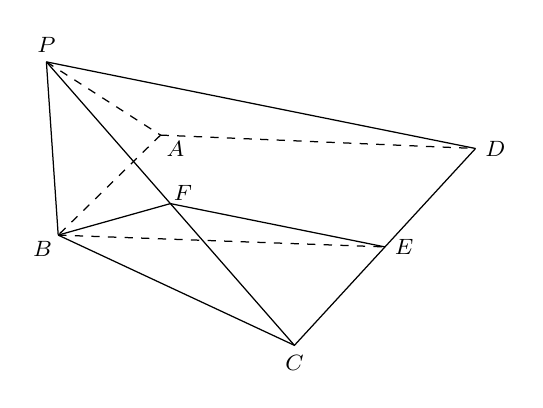
\begin{tikzpicture}[font=\footnotesize, line width=0.45pt]
  \coordinate (P) at (1.40,3.85);
  \coordinate (A) at (2.85,2.92);
  \coordinate (B) at (1.55,1.65);
  \coordinate (C) at (4.55,0.25);
  \coordinate (D) at (6.85,2.75);
  \coordinate (E) at (5.70,1.50);
  \coordinate (F) at (2.975,2.05);
  % 可见棱
  \draw (P) -- (B);
  \draw (P) -- (C);
  \draw (P) -- (D);
  \draw (B) -- (C) -- (D);
  \draw (B) -- (F) -- (E);
  % 被遮挡的棱
  \draw[dashed] (P) -- (A);
  \draw[dashed] (A) -- (B);
  \draw[dashed] (A) -- (D);
  \draw[dashed] (B) -- (E);
  % 顶点标注
  \node[above] at (P) {$P$};
  \node[below right, inner sep=2pt] at (A) {$A$};
  \node[below left, inner sep=2pt] at (B) {$B$};
  \node[below] at (C) {$C$};
  \node[right] at (D) {$D$};
  \node[right] at (E) {$E$};
  \node[above right, inner sep=1pt] at (F) {$F$};
\end{tikzpicture}
\end{center}
\nopagebreak[4]
\end{question}
\begin{question}
\gkti{18}已知函数 $f(x)=x^2+x\sin x+\cos x$。

（1） 若曲线 $y=f(x)$ 在点 $(a,f(a))$ 处与直线 $y=b$ 相切，求 $a$ 与 $b$ 的值；

（2） 若曲线 $y=f(x)$ 与直线 $y=b$ 有两个不同交点，求 $b$ 的取值范围。

\end{question}
\begin{question}
\gkti{19}直线 $y=kx+m$（$m\neq0$）与椭圆 $W:\dfrac{x^2}4+y^2=1$ 相交于 $A$，$C$ 两点，$O$ 是坐标原点。

（1） 当点 $B$ 的坐标为 $(0,1)$，且四边形 $OABC$ 为菱形时，求 $AC$ 的长；

（2） 当点 $B$ 在 $W$ 上且不是 $W$ 的顶点时，证明：四边形 $OABC$ 不可能为菱形。

\end{question}
\begin{question}
\gkti{20}给定数列 $a_1$，$a_2$，$\cdots$，$a_n$，对 $i=1$，$2$，$\cdots$，$n-1$，该数列前 $i$ 项的最大值记为 $A_i$，后 $n-i$ 项 $a_{i+1}$，$a_{i+2}$，$\cdots$，$a_n$ 的最小值记为 $B_i$，$d_i=A_i-B_i$。

（1） 设数列 $\{a_n\}$ 为 $3$，$4$，$7$，$1$，写出 $d_1$，$d_2$，$d_3$ 的值；

（2） 设 $a_1$，$a_2$，$\cdots$，$a_n$（$n\geqslant4$）是公比大于 $1$ 的等比数列，且 $a_1>0$。证明：$d_1$，$d_2$，$\cdots$，$d_{n-1}$ 是等比数列；

（3） 设 $d_1$，$d_2$，$\cdots$，$d_{n-1}$ 是公差大于 $0$ 的等差数列，且 $d_1>0$。证明：$a_1$，$a_2$，$\cdots$，$a_{n-1}$ 是等差数列。

\end{question}